\begin{appendix}

\section{Visualizing Errors : code chunk}
\label{appendix:visualizing}
\begin{lstlisting}[language=Python]
axes = plt.subplots(2, 4)[1]  # creates a grid of 10 plots

# More details about zip() function here https://docs.python.org/3.3/library/functions.html#zip
y_pred = clf4.predict(X_test)
j = 0 # Index which iterates over plots
for true_label, pred_label, image in list(zip(y_test, y_pred, X_test)):
    if j == 4: # We only want to look at 4 first mistakes
        break
    if true_label != pred_label:
        # Plotting predicted probabilities
        axes[1, j].bar(np.arange(10), clf4.predict_proba(image.reshape(1, -1))[0]) 
        axes[1, j].set_xticks(np.arange(10))
        axes[1, j].set_yticks([])
        
        # Plotting the image
        axes[0, j].imshow(image.reshape((28, 28)), cmap=plt.cm.gray_r, interpolation='nearest')
        axes[0, j].set_xticks([])
        axes[0, j].set_yticks([])
        axes[0, j].set_title('Predicted {}'.format(pred_label)+'/True {}'.format(true_label),fontsize=8)
        j += 1
\end{lstlisting}
	
\todo{maybe remove figure}
\begin{figure*}[h]
	\centering 
	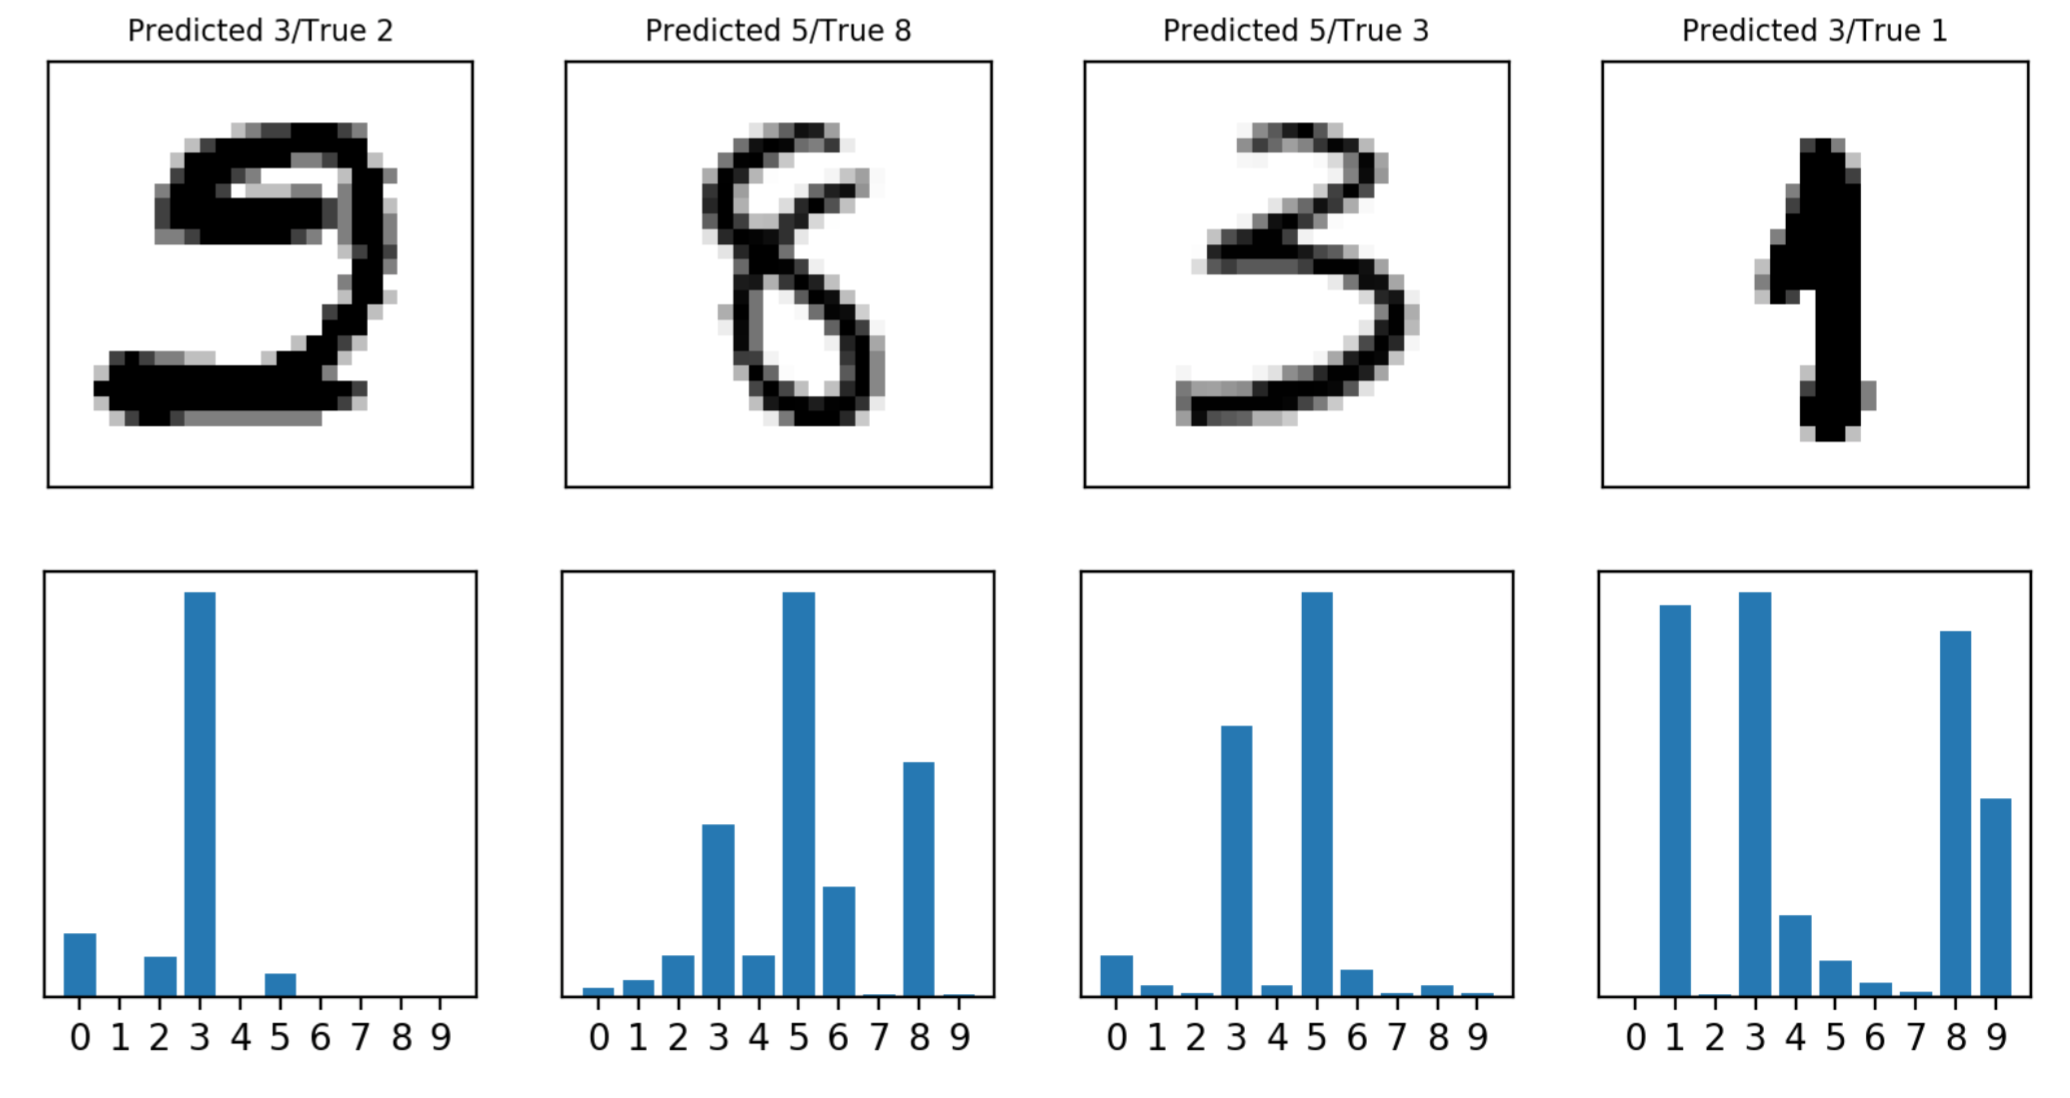
\includegraphics[scale=0.35]{Pics/probas}
	\caption{Probabilities of each outcome for the logistic regression}
	\label{fig:probas}
\end{figure*}

\end{appendix}

